% -*- TeX -*- -*- UK -*- -*- Soft -*-

\chapter{Activation Functions}
\label{sec:ActivationFunctions}

An activation function is usually a nonlinear (mathematical) function that transforms an input value (comprising the sum of a number of weighted input values and a bias) to an output value such that a non-trivial output range only appears over a given input domain. In other words, the output has significant value (not saturated at some limiting value) only for some limited scope of input values. 

Linear activations functions can also be used, mostly in the final output layer for regression, but generally linear activation functions are less useful than nonlinear activation functions.

The activation function is used at the output of a neural net perceptron to implement the perceptron functionality:
\begin{eqnarray}
\textrm{output} 
&=& \textrm{fn}\left(x_{1} w_{1}+x_{2} w_{2}+\cdots+x_{N} w_{N}+\textrm{bias}\right)\nonumber\\
&=& \textrm{fn}\left(\sum_{n=1}^N x_{n} w_{n}+\textrm{bias}\right)\nonumber.
\end{eqnarray}
The bias term offers the opportunity to `push' the sum into a region where the output has some significance relative to the input.

Several nonlinear functions are used in neural nets, including the sigmoid (logistics), tansig, or soft max
functions\cite{Pedamonti2018,Nwankpa2018,stackexchangeEllefsen2015,WikiPediaHyperbolicfunction2019,NickBecker2017,DustinStansbury2014,HamzaMahmood2018}. 

\section{Linear}

A linear function simply passes the signal with no change or compression
\begin{equation}
g(x)=kx.
\end{equation}  
The derivative of the linear function is the slope of the linear function
\begin{equation}
g^\prime(x) = k
\end{equation}
This function is linear and unbounded. The function is strictly increasing or decreasing (depending on the value of $k$). The function has little application except in cases where the linear output is specifically required.


\section{Logistic Sigmoid}

The sigmoid or logistics function is defined as (see Figure~\ref{fig:sigmoid}):
\begin{equation}
\sigma(x)
=\frac{1}{1+e^{-x}}.
\end{equation}  
The derivative of the sigmoid function is 
\begin{equation}
 \sigma^\prime(x)
 =\sigma(x)(1-\sigma(x))
\end{equation}
The notation $\textrm{sigm}()$ is sometimes used.
This function compresses the output bounded between 0 and 1, is always positive. The function is strictly increasing. Some recent research consider the logistic sigmoid function 'old-fashioned' and limited in value.

\begin{figure}[p]
\centering
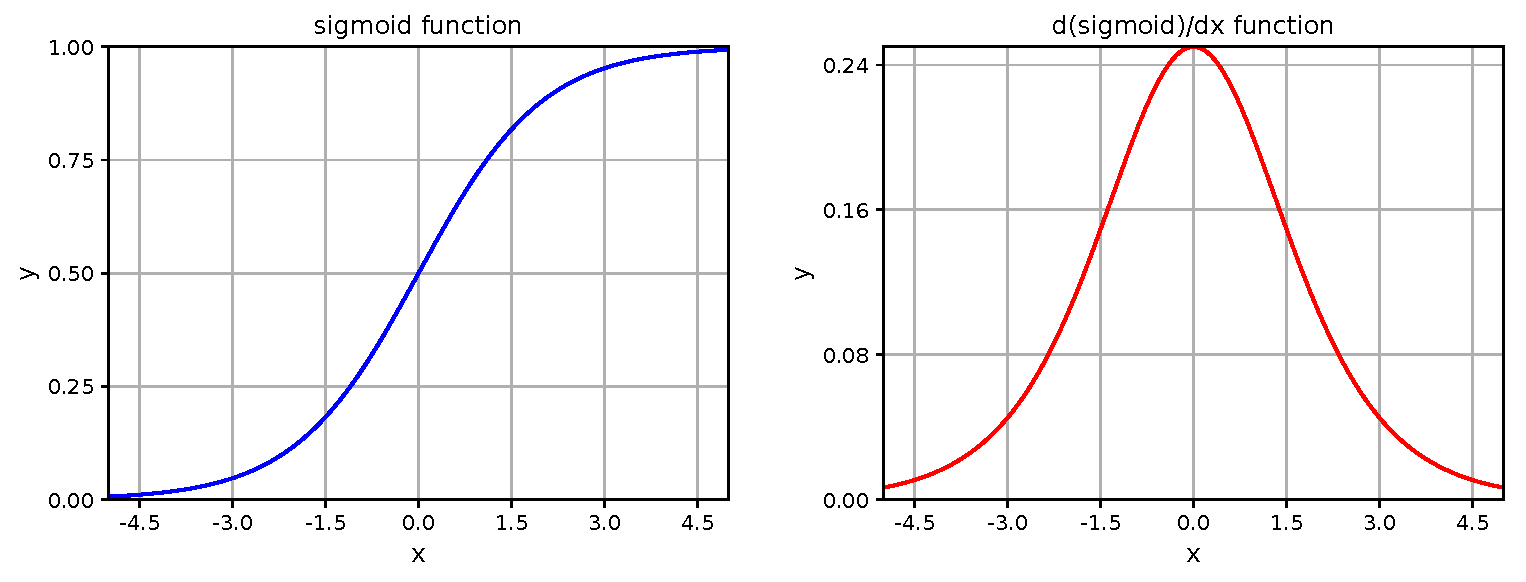
\includegraphics[width=\textwidth]{pic/sigmoid01}
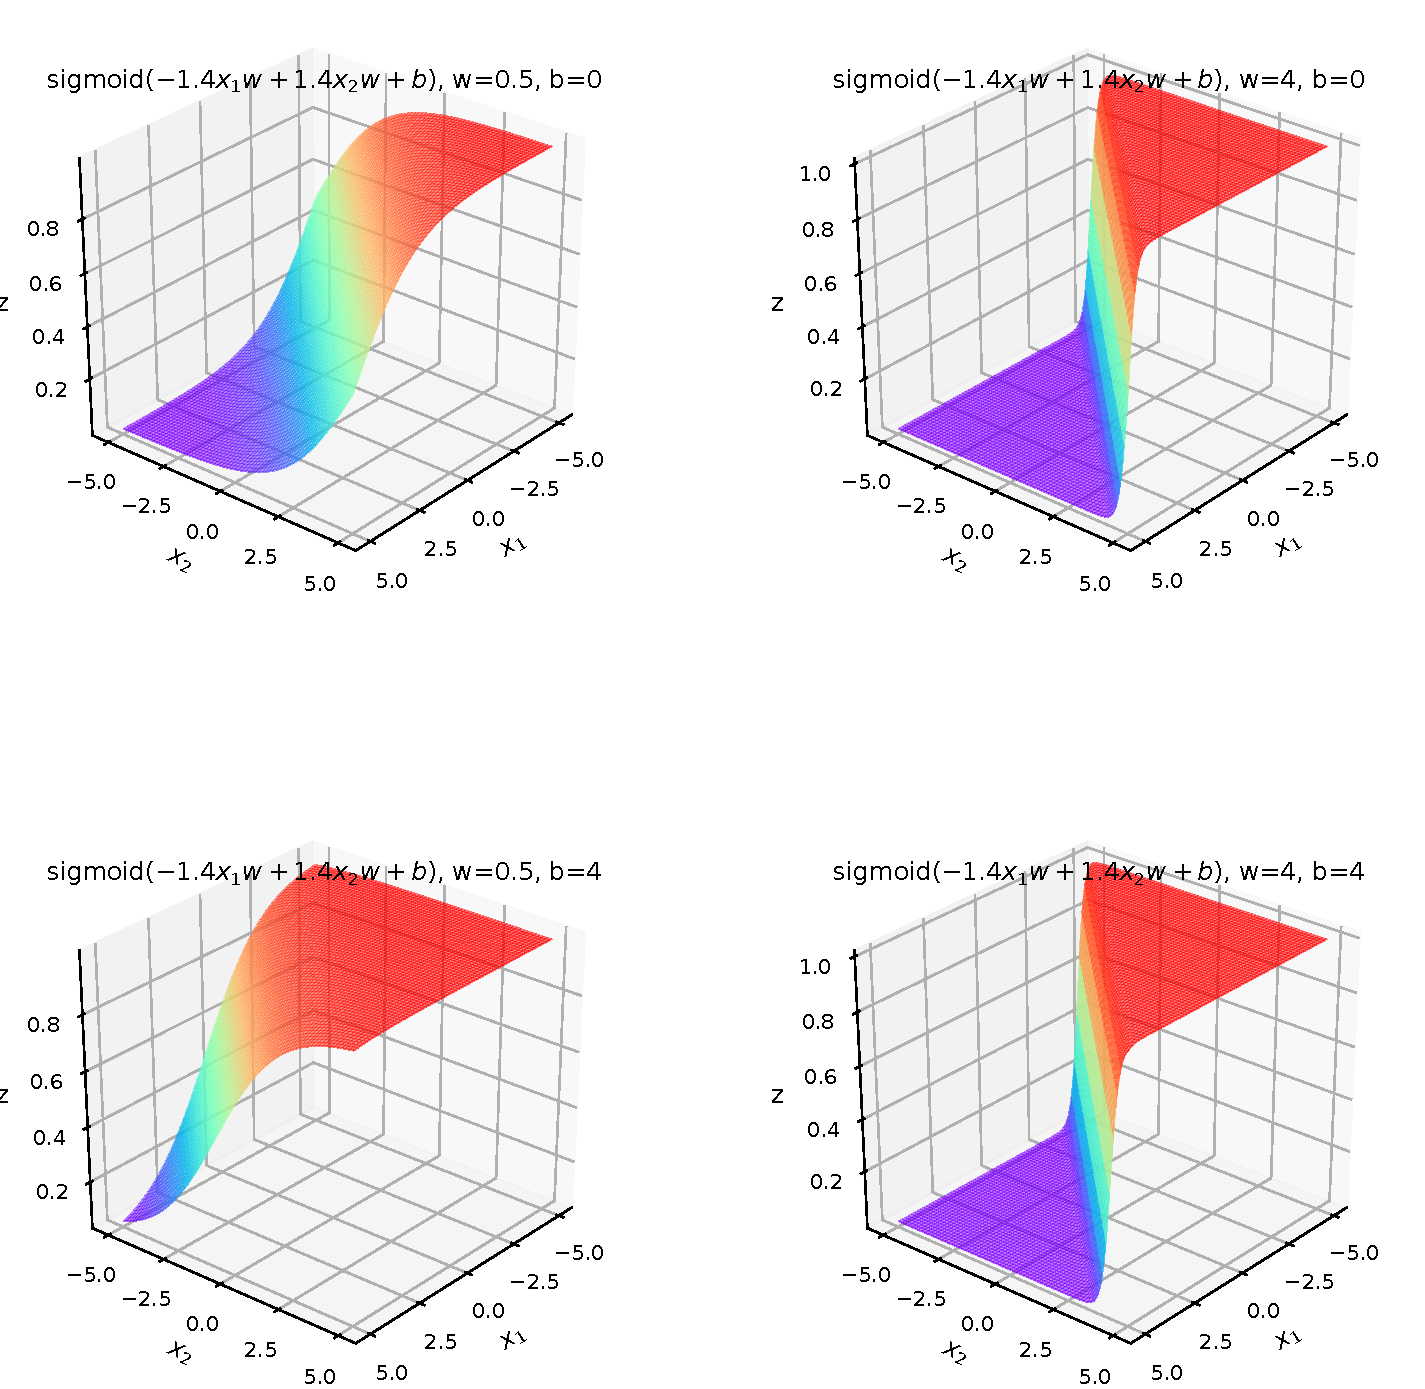
\includegraphics[width=\textwidth]{pic/sigmoid02}
\caption{The sigmoid function }
\label{fig:sigmoid}
\end{figure}


\section{Tansig or tanh}

The tansig function is defined as (see Figure~\ref{fig:tansig}):
\begin{equation}
\textrm{tanh}(x)
=\left(\frac{e^{x}-e^{-x}}{e^{x}+e^{-x}}\right)
=\left(\frac{e^{2x}-1}{e^{2x}+1}\right)
=\left(\frac{1-e^{-2x}}{1+e^{-2x}}\right)
=\left(\frac{2}{1+e^{-2x}}\right)-1,
\end{equation}  
but it is also sometimes seen in a (non-tanh) form:
\begin{equation}
\varphi(x)
=\left(\frac{1-e^{-bx}}{1+e^{-bx}}\right)
=\left(\frac{e^{bx}-1}{e^{bx}+1}\right)
=\left(\frac{2}{1+e^{-bx}}\right)-1
\end{equation}  
where, if $b=2$ yields the $\tanh(x)$ function.
The derivative of the tansig function is 
\begin{equation}
 \varphi^\prime(x)
 = \frac{b}{2} \left(1+\varphi(x))(1-\varphi(x)\right)
 = \frac{b}{2}\left(1-\varphi^2(x)\right)
\end{equation}
The notation $\textrm{tanh}()$ is sometimes used.
This function compresses the output bounded between -1 and 1. The function is strictly increasing. 



\begin{figure}[p]
\centering
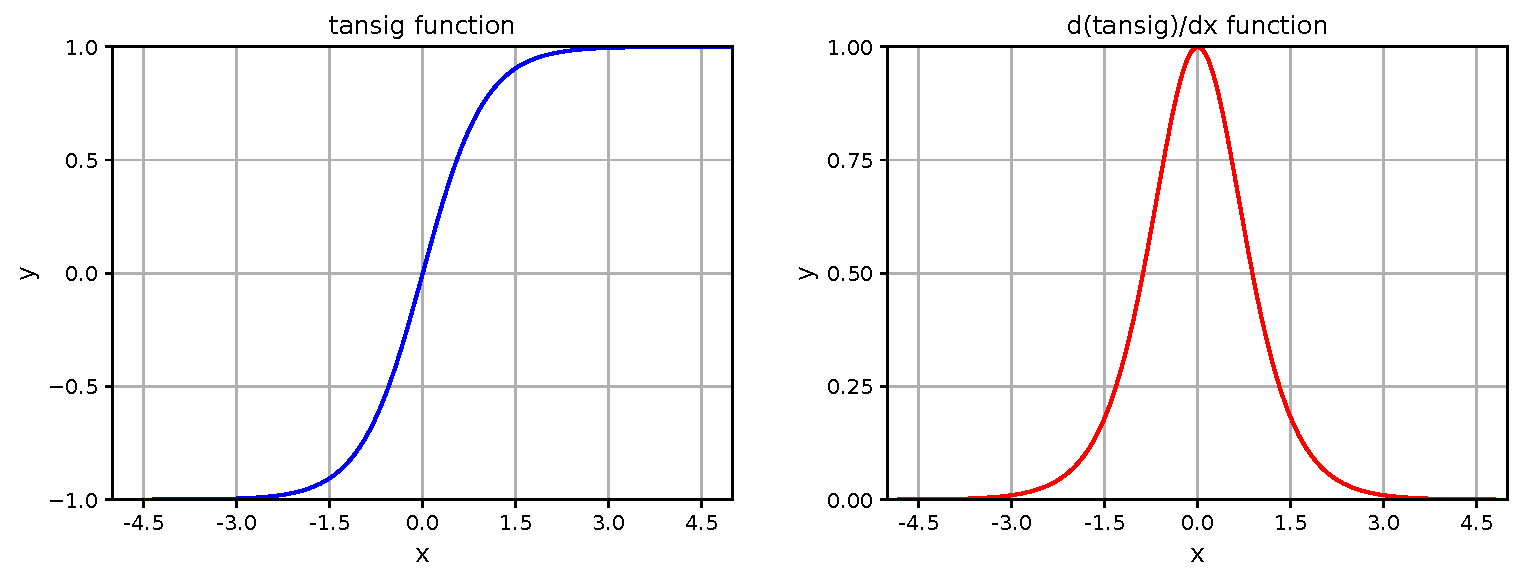
\includegraphics[width=\textwidth]{pic/tansig01}
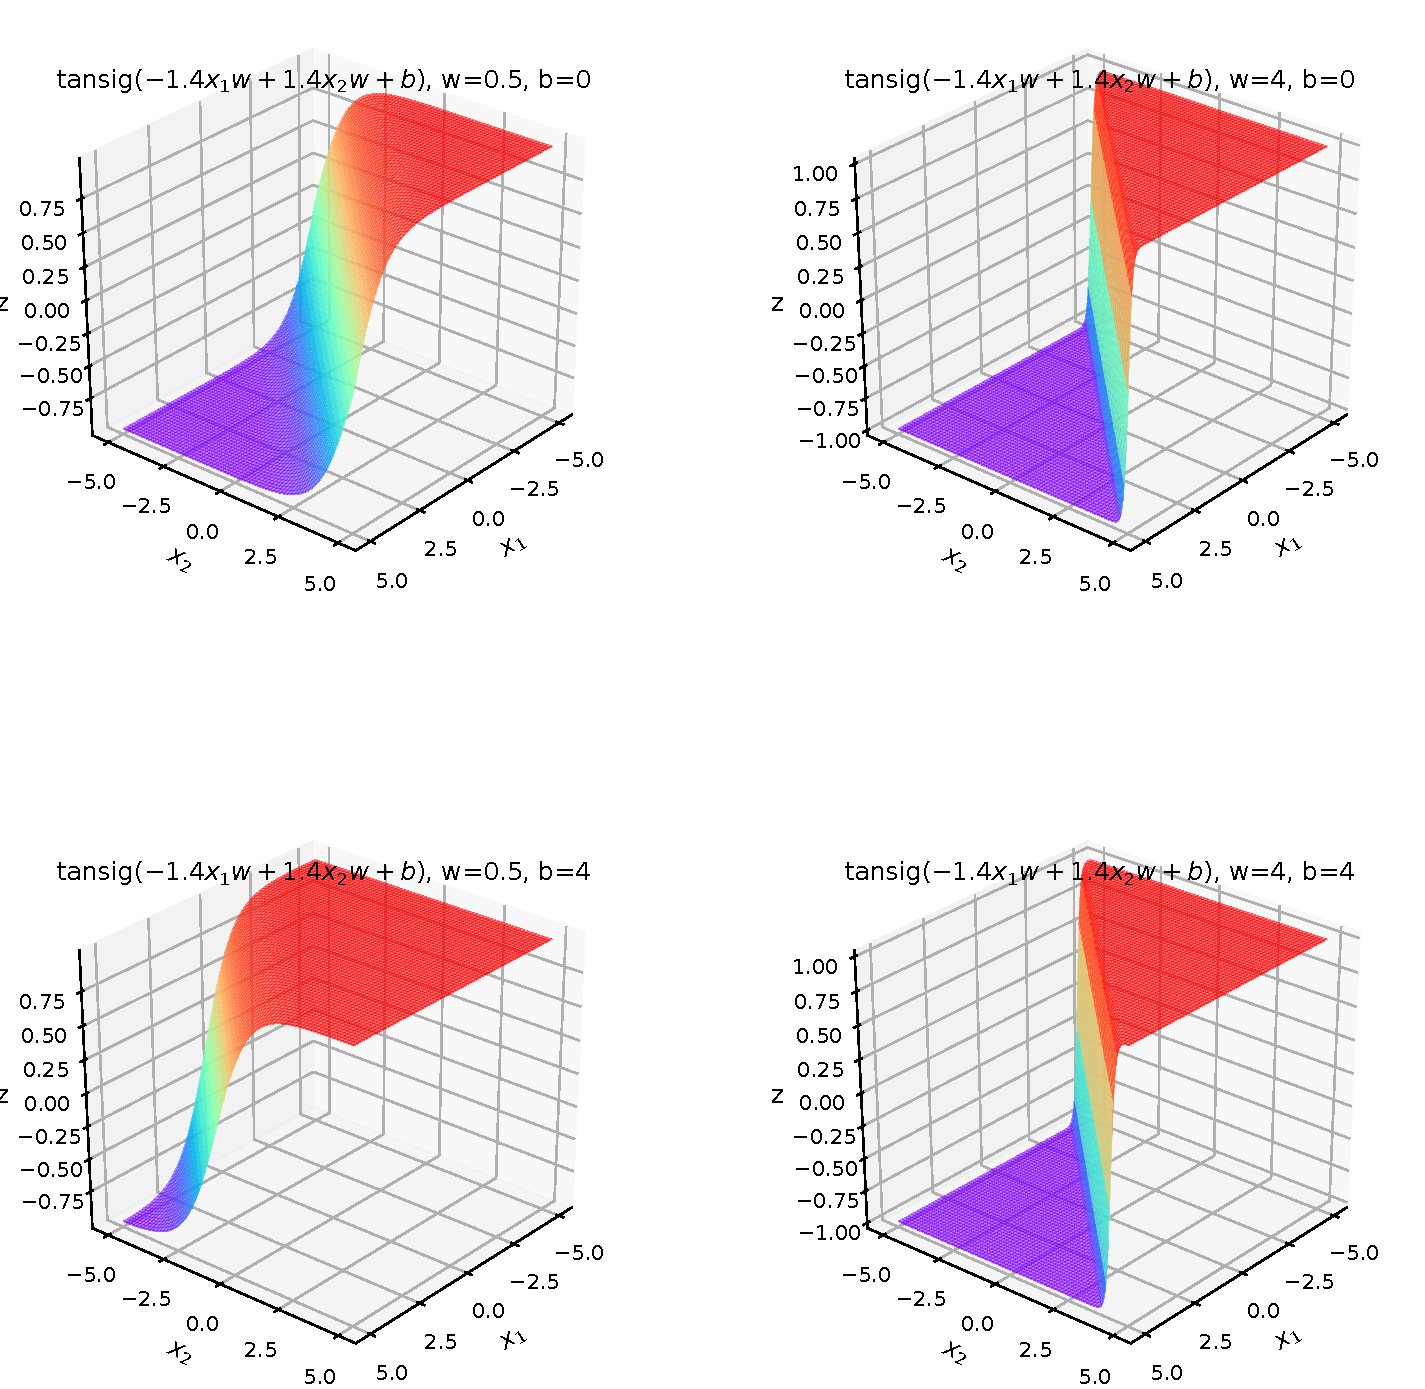
\includegraphics[width=\textwidth]{pic/tansig02}
\caption{The tansig function }
\label{fig:tansig}
\end{figure}



\section{Rectified Linear, RELU, or reclin}

The recently popular RELU/reclin function. mostly used in hidden layers, is defined as 
\begin{equation}
\textrm{reclin}(x) = \textrm{max}(0,kx)
\end{equation}
The reclin function is bounded below by 0, it is always non-negative, but has no upper bound.  This function tends to result in neurons with sparse activity, in this case 0 output for all negative inputs.


\section{Softmax}
\label{sec:c10-softmax}
The softmax (also known as the Boltzmann distribution or the normalised exponential transformation) function takes as input a vector of $K$ real numbers, and normalizes it into a probability distribution consisting of $K$ probabilities. 
The WikiPedia page  \cite{WikiPediaSoftmaxFunction2019} has a good description of this function.

Prior to applying softmax, some vector components could be negative, or greater than one; and might not sum to 1; but after applying softmax, each component will be in the interval (0,1), and the components will add up to 1, so that they can be interpreted as probabilities. Furthermore, the larger input components will correspond to larger probabilities. Softmax is used to map the non-normalized output of a network to a probability distribution over predicted output classes. 
It is defined as \cite{WikiPediaSoftmaxFunction2019,HamzaMahmood2018}

\begin{equation}
\sigma(\mathbf{x})_{i}=\frac{e^{x_{i}}}{\sum_{j=1}^{K} e^{x_{j}}} \quad \text { for } i=1, \ldots, K \text { and } \mathbf{x}=\left(x_{1}, \ldots, x_{K}\right) \in \mathbb{R}^{K}
\end{equation}

Apply the standard exponential function to each element $x_i$  of the input vector $\mathbf{x}$ and normalize these values by dividing by the sum of all these exponentials; this normalization ensures that the sum of the components of the output vector $\sigma(\mathbf {z}$ is 1. 
Instead of $e$, a different base $b>0$ can be used; choosing a larger value of $b$ will create a probability distribution that is more concentrated around the positions of the largest input values. 

The softmax function is often used in the final layer of a neural network-based classifier. Such networks are commonly trained under a log loss (or cross-entropy) regime, giving a non-linear variant of multinomial logistic regression.

Since the function maps a vector and a specific index $i$ to a real value, the derivative needs to take the index into account: 
\begin{equation}
\frac{\partial}{\partial q_{k}} \sigma(\mathbf{q}, i)=\cdots=\sigma(\mathbf{q}, i)\left(\delta_{i k}-\sigma(\mathbf{q}, k)\right)
\end{equation}

There is no graph of this function, but consider the following example from \cite{WikiPediaSoftmaxFunction2019}.
If we take an input of \lstinline{[1, 2, 3, 4, 1, 2, 3]}, the softmax of that is \lstinline{[0.024, 0.064, 0.175, 0.475, 0.024, 0.064, 0.175]}. The output has most of its weight where the \lstinline{4} was in the original input. This is what the function is normally used for: to highlight the largest values and suppress values which are significantly below the maximum value. But note: softmax is not scale invariant, so if the input were \lstinline{[0.1, 0.2, 0.3, 0.4, 0.1, 0.2, 0.3]} (which sums to \lstinline{1.6}) the softmax would be \lstinline{[0.125, 0.138, 0.153, 0.169, 0.125, 0.138, 0.153]}. This shows that for values between 0 and 1 softmax, in fact, de-emphasizes the maximum value (note that \lstinline{0.169} is not only less than \lstinline{0.475}, it is also less than the initial proportion of \lstinline{0.4/1.6=0.25}). 
\begin{lstlisting}
>>> import math
>>> z = [1.0, 2.0, 3.0, 4.0, 1.0, 2.0, 3.0]
>>> z_exp = [math.exp(i) for i in z]
>>> print([round(i, 2) for i in z_exp])
[2.72, 7.39, 20.09, 54.6, 2.72, 7.39, 20.09]
>>> sum_z_exp = sum(z_exp)
>>> print(round(sum_z_exp, 2))
114.98
>>> softmax = [i / sum_z_exp for i in z_exp]
>>> print([round(i, 3) for i in softmax])
[0.024, 0.064, 0.175, 0.475, 0.024, 0.064, 0.175]
\end{lstlisting}



An interactive example of the softmax function is implemented in the notebook at
\lstinline{../code/chapter3-graphics.ipynb}.}.  The code, running in the Jupyter notebook, is as follows:
\begin{marginfigure}[-80mm]
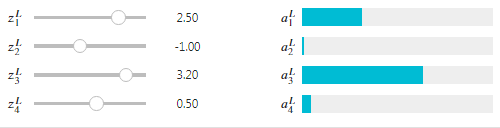
\includegraphics{ch03-snip06}
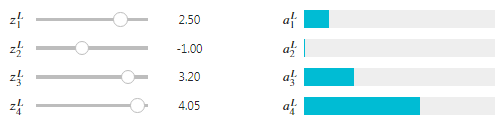
\includegraphics{ch03-snip07}
\end{marginfigure}
\begin{lstlisting}
import numpy as np
from ipywidgets import HBox,VBox,Button,FloatSlider,FloatProgress,interactive

# set up the widgets with precalculated values
# these sliders and prog bars are visible and are updated below in the softmax function
sliders = {'1':[2.5,0.31], '2':[-1.,0.009], '3':[3.2,0.633], '4':[0.5,0.043]}
sld = {key:FloatSlider(min=-5.0, max=+5.0, value=f'{sliders[key][0]}', step=0.05,description=f'$z^L_{key}$') for key in sliders}
prb = {key:FloatProgress(value=f'{sliders[key][1]}',min=0,max=1.0,step=0.01,description=f'$a^L_{key}$',bar_style='info',orientation='horizontal') for key in sliders}

# build and display the widget grid in pairs of sliders and prog bars
lstD = [HBox([sld[key], prb[key]]) for key in sld]
display(VBox(lstD))

# function is invoked if any of the sliders change
# and the result is used to change the progress bar
def softmax(**lstZ):
    sum = 0
    for key in lstZ:
        sum += np.exp(lstZ[key])
    for key in lstZ:
        prb[key].value = np.exp(lstZ[key])/sum

#  `interactive` does not display/show the widgets, already done above.
w = interactive(softmax, **sld )
\end{lstlisting}

\TBC{todo}
\begin{lstlisting}

https://towardsdatascience.com/softmax-function-simplified-714068bf8156

https://theclevermachine.wordpress.com/2014/09/08/derivation-derivatives-for-common-neural-network-activation-functions/

https://towardsdatascience.com/interpretable-neural-networks-45ac8aa91411

https://stats.stackexchange.com/questions/48470/interpreting-the-output-of-a-neural-network

https://dsotb.quora.com/Deep-learning-with-Keras-convolutional-neural-networks-demystified
\end{lstlisting} 